\chapter{Installation}
\label{chp:installation}
The \ProductName{} PyQt Windows interface \IfXi{is provided as a standard installation EXE file.}
\IfGNU{is provided as a collection of Python Source files. It can be run on GNU/Linux using PyQT or it can be run on Windows with
Python, PyQt and the Python Win 32 API interface}.

Before starting, we suggest that you first set up the Unix hosts as explained in the Administration Manual according to whether the PCs have fixed IP
addresses or are DHCP clients.

The copies of \ProductName{} on the Unix hosts should be set up to be ``networked'', i.e. so that jobs and variables are
shared across the network. It would be helpful if the local name services can resolve names to the relevant IPs, but this is not
essential.

\IfXi{Run the installation program provided, selecting the desired path required for the binaries. You may opt to include the desktop
icons or not as required.}

Unlike the Visual C++ version, there are only two programs to be installed, \progname{btqw} and \progname{btrw}, not three, i.e. there is
no \progname{btrsetw}. The facilities formerly provided by \progname{btrsetw} are provided in \progname{btqw}. However the other
functionalities of \progname{btqw} and \progname{btrw} are similar.

A key difference between the two versions of the MS Clients are that saved jobs are now held in a single file in XML format rather than
having a saved script and a separate job file.

\IfXi{\section{Running the install program}

The installation suite is provided as a Windows executable which may be run to install the software in the default or a user-chosen
directory and optionally to provide desktop links to the \progname{btqw} and \progname{btrw} programs.

On completion of installation, \progname{btqw} is entered, and the user can commence the initial setup.}

\IfGNU{\section{Starting up}

We suggest you start by running the \progname{btqw} as the Python file \filename{btqw.py}. You may need to resolve some missing dependencies.}

When first entered, the display will look like the following:

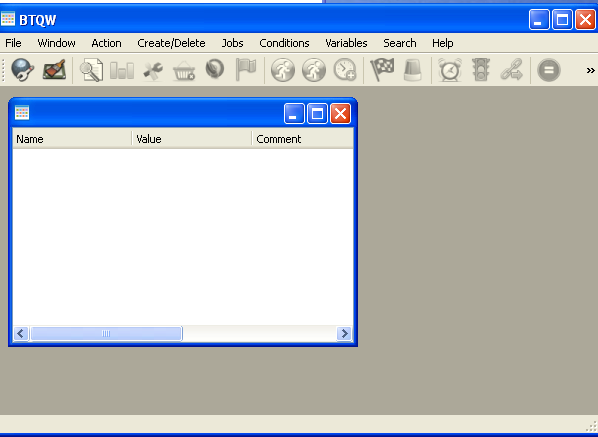
\includegraphics{img/btqwinit.png}

To set up the servers, select the \textbf{Server list} item from the \textbf{File} menu.

The following dialog box should be displayed

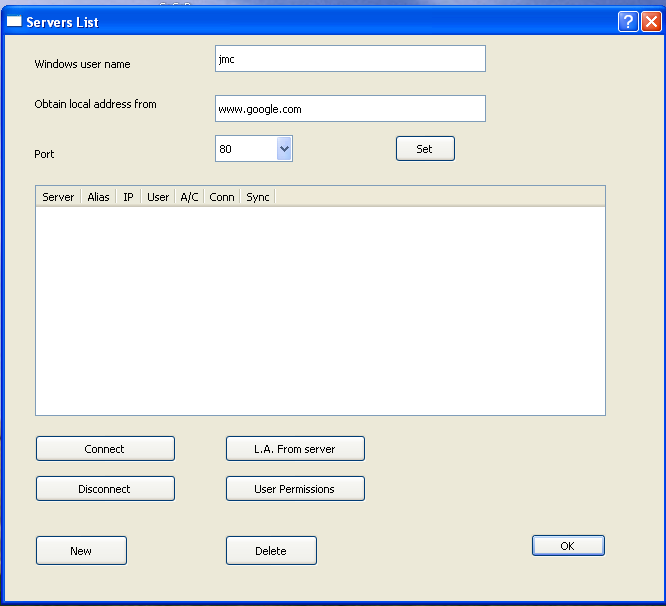
\includegraphics{img/btqwservinit.png}

\subsection{Setting the local address}

The first task will be to set up to interrogate the local IP address. This is important in order to distinguish references to the local machine
(i.e. the Windows client) from other IP addresses. This is usually done by making a connection to some web site and looking at the
local address.

When first set up, the web site \filename{www.google.com} is set up, but this can be changed to any other. When ready, press the \textbf{Set}
button to initialise the local address. If this runs satisfactorily, it will be used henceforth.

\subsection{Setting the server address}
\label{bkm:installservs}

To set up one or more servers, click the \textbf{New} button, to receive the dialog box:

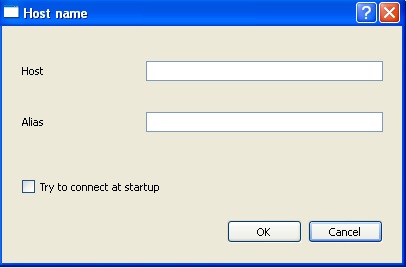
\includegraphics{img/btqwnewhost.png}

In the \textbf{Host} box put either the server name, if it is recognised by the domain name system, or else the server IP address.

If the server is given as an IP address, put a suitable alias name, we suggest one or two characters, by which the server will be referenced
on all the windows and dialog boxes in \progname{btqw} or \progname{btrw}. You can also do this to provide a convenient abbreviation for the
server name if you wish.

You will usually want to indicate that you want the server to be connected every time you start up \progname{btqw}, in which case you should
set the checkbox given, for example:

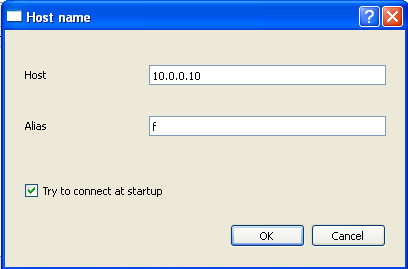
\includegraphics{img/btqwnewhostset.png}

When done, press OK and the program returns to the previous dialog with the server details filled in, thus:

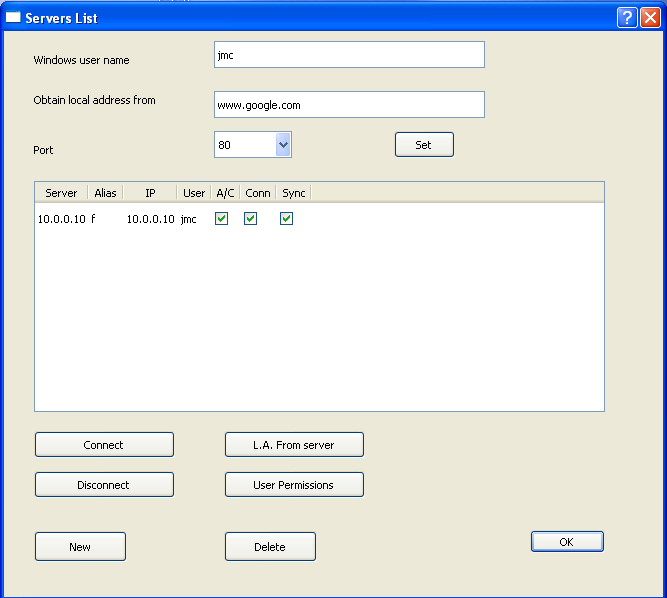
\includegraphics{img/btqwnewhostsetlist.png}

If this looks correct, select the line by clicking on it and press the \textbf{Connect} button.

You will probably get a dialog like this:

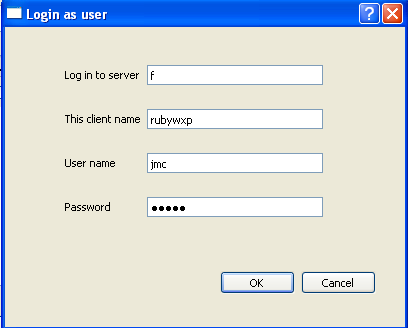
\includegraphics{img/btqwlogin.png}

You may need to edit the login name (although the server may have been set to map Windows user names to UNIX ones) and put your password in
(although you can set a password for \ProductName{} different from your login password on the server if you want to using \PrXipasswd).

After successfully logging in, quit from the server setup dialog and the exported jobs and variables should appear on the two windows initially
displayed.

Initially one job window and one variable window is displayed and you may want to move these apart and resize them.

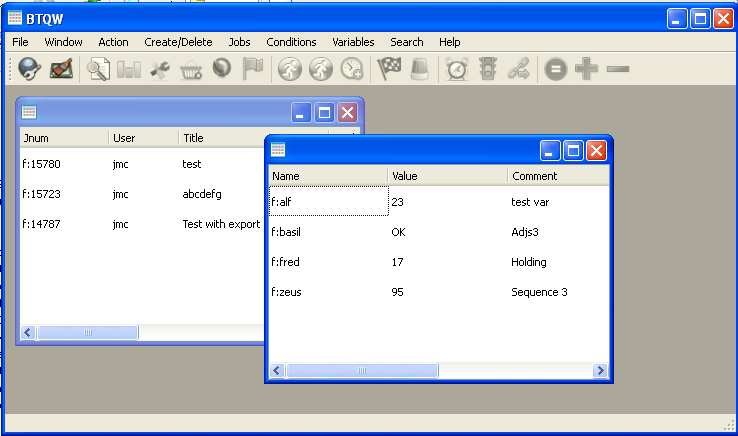
\includegraphics{img/btqwjwfirst.png}

The settings and the dimensions of the windows are saved when \progname{btqw} is exited and restored next time.


